\documentclass[12pt]{article}

%packages
%\usepackage{latexsym}
\usepackage{graphicx}
\usepackage{color}
\usepackage{amsmath}
\usepackage{dsfont}
\usepackage{placeins}
\usepackage{amssymb}
\usepackage{wasysym}
\usepackage{abstract}
\usepackage{hyperref}
\usepackage{etoolbox}
\usepackage{datetime}
\usepackage{xcolor}
\usepackage{alphalph}
\settimeformat{ampmtime}

%\usepackage{pstricks,pst-node,pst-tree}

%\usepackage{algpseudocode}
%\usepackage{amsthm}
%\usepackage{hyperref}
%\usepackage{mathrsfs}
%\usepackage{amsfonts}
%\usepackage{bbding}
%\usepackage{listings}
%\usepackage{appendix}
\usepackage[margin=1in]{geometry}
%\geometry{papersize={8.5in,11in},total={6.5in,9in}}
%\usepackage{cancel}
%\usepackage{algorithmic, algorithm}

\makeatletter
\def\maxwidth{ %
  \ifdim\Gin@nat@width>\linewidth
    \linewidth
  \else
    \Gin@nat@width
  \fi
}
\makeatother

\definecolor{fgcolor}{rgb}{0.345, 0.345, 0.345}
\newcommand{\hlnum}[1]{\textcolor[rgb]{0.686,0.059,0.569}{#1}}%
\newcommand{\hlstr}[1]{\textcolor[rgb]{0.192,0.494,0.8}{#1}}%
\newcommand{\hlcom}[1]{\textcolor[rgb]{0.678,0.584,0.686}{\textit{#1}}}%
\newcommand{\hlopt}[1]{\textcolor[rgb]{0,0,0}{#1}}%
\newcommand{\hlstd}[1]{\textcolor[rgb]{0.345,0.345,0.345}{#1}}%
\newcommand{\hlkwa}[1]{\textcolor[rgb]{0.161,0.373,0.58}{\textbf{#1}}}%
\newcommand{\hlkwb}[1]{\textcolor[rgb]{0.69,0.353,0.396}{#1}}%
\newcommand{\hlkwc}[1]{\textcolor[rgb]{0.333,0.667,0.333}{#1}}%
\newcommand{\hlkwd}[1]{\textcolor[rgb]{0.737,0.353,0.396}{\textbf{#1}}}%

\usepackage{framed}
\makeatletter
\newenvironment{kframe}{%
 \def\at@end@of@kframe{}%
 \ifinner\ifhmode%
  \def\at@end@of@kframe{\end{minipage}}%
  \begin{minipage}{\columnwidth}%
 \fi\fi%
 \def\FrameCommand##1{\hskip\@totalleftmargin \hskip-\fboxsep
 \colorbox{shadecolor}{##1}\hskip-\fboxsep
     % There is no \\@totalrightmargin, so:
     \hskip-\linewidth \hskip-\@totalleftmargin \hskip\columnwidth}%
 \MakeFramed {\advance\hsize-\width
   \@totalleftmargin\z@ \linewidth\hsize
   \@setminipage}}%
 {\par\unskip\endMakeFramed%
 \at@end@of@kframe}
\makeatother

\definecolor{shadecolor}{rgb}{.77, .77, .77}
\definecolor{messagecolor}{rgb}{0, 0, 0}
\definecolor{warningcolor}{rgb}{1, 0, 1}
\definecolor{errorcolor}{rgb}{1, 0, 0}
\newenvironment{knitrout}{}{} % an empty environment to be redefined in TeX

\usepackage{alltt}
\usepackage[T1]{fontenc}

\newcommand{\qu}[1]{``#1''}
\newcounter{probnum}
\setcounter{probnum}{1}

%create definition to allow local margin changes
\def\changemargin#1#2{\list{}{\rightmargin#2\leftmargin#1}\item[]}
\let\endchangemargin=\endlist 

%allow equations to span multiple pages
\allowdisplaybreaks

%define colors and color typesetting conveniences
\definecolor{gray}{rgb}{0.5,0.5,0.5}
\definecolor{black}{rgb}{0,0,0}
\definecolor{white}{rgb}{1,1,1}
\definecolor{blue}{rgb}{0.5,0.5,1}
\newcommand{\inblue}[1]{\color{blue}#1 \color{black}}
\definecolor{green}{rgb}{0.133,0.545,0.133}
\newcommand{\ingreen}[1]{\color{green}#1 \color{black}}
\definecolor{yellow}{rgb}{1,1,0}
\newcommand{\inyellow}[1]{\color{yellow}#1 \color{black}}
\definecolor{orange}{rgb}{0.9,0.649,0}
\newcommand{\inorange}[1]{\color{orange}#1 \color{black}}
\definecolor{red}{rgb}{1,0.133,0.133}
\newcommand{\inred}[1]{\color{red}#1 \color{black}}
\definecolor{purple}{rgb}{0.58,0,0.827}
\newcommand{\inpurple}[1]{\color{purple}#1 \color{black}}
\definecolor{backgcode}{rgb}{0.97,0.97,0.8}
\definecolor{Brown}{cmyk}{0,0.81,1,0.60}
\definecolor{OliveGreen}{cmyk}{0.64,0,0.95,0.40}
\definecolor{CadetBlue}{cmyk}{0.62,0.57,0.23,0}

%define new math operators
\DeclareMathOperator*{\argmax}{arg\,max~}
\DeclareMathOperator*{\argmin}{arg\,min~}
\DeclareMathOperator*{\argsup}{arg\,sup~}
\DeclareMathOperator*{\arginf}{arg\,inf~}
\DeclareMathOperator*{\convolution}{\text{\Huge{$\ast$}}}
\newcommand{\infconv}[2]{\convolution^\infty_{#1 = 1} #2}
%true functions

%%%% GENERAL SHORTCUTS

%shortcuts for pure typesetting conveniences
\newcommand{\bv}[1]{\boldsymbol{#1}}

%shortcuts for compound constants
\newcommand{\BetaDistrConst}{\dfrac{\Gamma(\alpha + \beta)}{\Gamma(\alpha)\Gamma(\beta)}}
\newcommand{\NormDistrConst}{\dfrac{1}{\sqrt{2\pi\sigma^2}}}

%shortcuts for conventional symbols
\newcommand{\tsq}{\tau^2}
\newcommand{\tsqh}{\hat{\tau}^2}
\newcommand{\sigsq}{\sigma^2}
\newcommand{\sigsqsq}{\parens{\sigma^2}^2}
\newcommand{\sigsqovern}{\dfrac{\sigsq}{n}}
\newcommand{\tausq}{\tau^2}
\newcommand{\tausqalpha}{\tau^2_\alpha}
\newcommand{\tausqbeta}{\tau^2_\beta}
\newcommand{\tausqsigma}{\tau^2_\sigma}
\newcommand{\betasq}{\beta^2}
\newcommand{\sigsqvec}{\bv{\sigma}^2}
\newcommand{\sigsqhat}{\hat{\sigma}^2}
\newcommand{\sigsqhatmlebayes}{\sigsqhat_{\text{Bayes, MLE}}}
\newcommand{\sigsqhatmle}[1]{\sigsqhat_{#1, \text{MLE}}}
\newcommand{\bSigma}{\bv{\Sigma}}
\newcommand{\bSigmainv}{\bSigma^{-1}}
\newcommand{\thetavec}{\bv{\theta}}
\newcommand{\thetahat}{\hat{\theta}}
\newcommand{\thetahatmle}{\hat{\theta}_{\mathrm{MLE}}}
\newcommand{\thetavechatmle}{\hat{\thetavec}_{\mathrm{MLE}}}
\newcommand{\muhat}{\hat{\mu}}
\newcommand{\musq}{\mu^2}
\newcommand{\muvec}{\bv{\mu}}
\newcommand{\muhatmle}{\muhat_{\text{MLE}}}
\newcommand{\lambdahat}{\hat{\lambda}}
\newcommand{\lambdahatmle}{\lambdahat_{\text{MLE}}}
\newcommand{\etavec}{\bv{\eta}}
\newcommand{\alphavec}{\bv{\alpha}}
\newcommand{\minimaxdec}{\delta^*_{\mathrm{mm}}}
\newcommand{\ybar}{\bar{y}}
\newcommand{\xbar}{\bar{x}}
\newcommand{\Xbar}{\bar{X}}
\newcommand{\phat}{\hat{p}}
\newcommand{\Phat}{\hat{P}}
\newcommand{\Zbar}{\bar{Z}}
\newcommand{\iid}{~{\buildrel iid \over \sim}~}
\newcommand{\inddist}{~{\buildrel ind \over \sim}~}
\newcommand{\approxdist}{~{\buildrel approx \over \sim}~}
\newcommand{\equalsindist}{~{\buildrel d \over =}~}
\newcommand{\loglik}[1]{\ell\parens{#1}}
\newcommand{\thetahatkminone}{\thetahat^{(k-1)}}
\newcommand{\thetahatkplusone}{\thetahat^{(k+1)}}
\newcommand{\thetahatk}{\thetahat^{(k)}}
\newcommand{\half}{\frac{1}{2}}
\newcommand{\third}{\frac{1}{3}}
\newcommand{\twothirds}{\frac{2}{3}}
\newcommand{\fourth}{\frac{1}{4}}
\newcommand{\fifth}{\frac{1}{5}}
\newcommand{\sixth}{\frac{1}{6}}

%shortcuts for vector and matrix notation
\newcommand{\A}{\bv{A}}
\renewcommand{\b}{\bv{b}}
\newcommand{\w}{\bv{w}}
\newcommand{\At}{\A^T}
\newcommand{\Ainv}{\inverse{\A}}
\newcommand{\B}{\bv{B}}
\newcommand{\K}{\bv{K}}
\newcommand{\Kt}{\K^T}
\newcommand{\Kinv}{\inverse{K}}
\newcommand{\Kinvt}{(\Kinv)^T}
\newcommand{\M}{\bv{M}}
\newcommand{\Bt}{\B^T}
\newcommand{\Q}{\bv{Q}}
\newcommand{\Qt}{\Q^T}
\newcommand{\R}{\bv{R}}
\newcommand{\Rt}{\R^T}
\newcommand{\Z}{\bv{Z}}
\newcommand{\X}{\bv{X}}
\newcommand{\Xsub}{\X_{\text{(sub)}}}
\newcommand{\Xsubadj}{\X_{\text{(sub,adj)}}}
\newcommand{\I}{\bv{I}}
\newcommand{\Y}{\bv{Y}}
\newcommand{\sigsqI}{\sigsq\I}
\renewcommand{\P}{\bv{P}}
\newcommand{\Psub}{\P_{\text{(sub)}}}
\newcommand{\Pt}{\P^T}
\newcommand{\Pii}{P_{ii}}
\newcommand{\Pij}{P_{ij}}
\newcommand{\IminP}{(\I-\P)}
\newcommand{\Xt}{X^\top}
\newcommand{\XtX}{\Xt X}
\newcommand{\XtXinv}{\parens{\Xt X}^{-1}}
\newcommand{\XtXinvXt}{\XtXinv\Xt}
\newcommand{\XXtXinvXt}{X\XtXinvXt}
\newcommand{\x}{\bv{x}}
\newcommand{\onevec}{\bv{1}}
\newcommand{\zerovec}{\bv{0}}
\newcommand{\oneton}{1, \ldots, n}
\newcommand{\yoneton}{y_1, \ldots, y_n}
\newcommand{\yonetonorder}{y_{(1)}, \ldots, y_{(n)}}
\newcommand{\Yoneton}{Y_1, \ldots, Y_n}
\newcommand{\iinoneton}{i \in \braces{\oneton}}
\newcommand{\onetom}{1, \ldots, m}
\newcommand{\jinonetom}{j \in \braces{\onetom}}
\newcommand{\xoneton}{x_1, \ldots, x_n}
\newcommand{\Xoneton}{X_1, \ldots, X_n}
\newcommand{\xt}{\x^T}
\newcommand{\y}{\bv{y}}
\newcommand{\yt}{\y^T}
\renewcommand{\c}{\bv{c}}
\newcommand{\ct}{\c^T}
\newcommand{\tstar}{\bv{t}^*}
\renewcommand{\u}{\bv{u}}
\renewcommand{\v}{\bv{v}}
\renewcommand{\a}{\bv{a}}
\newcommand{\s}{\bv{s}}
\newcommand{\yadj}{\y_{\text{(adj)}}}
\newcommand{\xjadj}{\x_{j\text{(adj)}}}
\newcommand{\xjadjM}{\x_{j \perp M}}
\newcommand{\yhat}{\hat{\y}}
\newcommand{\yhatsub}{\yhat_{\text{(sub)}}}
\newcommand{\yhatstar}{\yhat^*}
\newcommand{\yhatstarnew}{\yhatstar_{\text{new}}}
\newcommand{\z}{\bv{z}}
\newcommand{\zt}{\z^T}
\newcommand{\bb}{\bv{b}}
\newcommand{\bbt}{\bb^T}
\newcommand{\bbeta}{\bv{\beta}}
\newcommand{\beps}{\bv{\epsilon}}
\newcommand{\bepst}{\beps^T}
\newcommand{\e}{\bv{e}}
\newcommand{\Mofy}{\M(\y)}
\newcommand{\KofAlpha}{K(\alpha)}
\newcommand{\ellset}{\mathcal{L}}
\newcommand{\oneminalph}{1-\alpha}
\newcommand{\SSE}{\text{SSE}}
\newcommand{\SSEsub}{\text{SSE}_{\text{(sub)}}}
\newcommand{\MSE}{\text{MSE}}
\newcommand{\RMSE}{\text{RMSE}}
\newcommand{\SSR}{\text{SSR}}
\newcommand{\SST}{\text{SST}}
\newcommand{\JSest}{\delta_{\text{JS}}(\x)}
\newcommand{\Bayesest}{\delta_{\text{Bayes}}(\x)}
\newcommand{\EmpBayesest}{\delta_{\text{EmpBayes}}(\x)}
\newcommand{\BLUPest}{\delta_{\text{BLUP}}}
\newcommand{\MLEest}[1]{\hat{#1}_{\text{MLE}}}

%shortcuts for Linear Algebra stuff (i.e. vectors and matrices)
\newcommand{\twovec}[2]{\bracks{\begin{array}{c} #1 \\ #2 \end{array}}}
\newcommand{\threevec}[3]{\bracks{\begin{array}{c} #1 \\ #2 \\ #3 \end{array}}}
\newcommand{\fivevec}[5]{\bracks{\begin{array}{c} #1 \\ #2 \\ #3 \\ #4 \\ #5 \end{array}}}
\newcommand{\twobytwomat}[4]{\bracks{\begin{array}{cc} #1 & #2 \\ #3 & #4 \end{array}}}
\newcommand{\threebytwomat}[6]{\bracks{\begin{array}{cc} #1 & #2 \\ #3 & #4 \\ #5 & #6 \end{array}}}


%shortcuts for conventional compound symbols
\newcommand{\thetainthetas}{\theta \in \Theta}
\newcommand{\reals}{\mathbb{R}}
\newcommand{\complexes}{\mathbb{C}}
\newcommand{\rationals}{\mathbb{Q}}
\newcommand{\integers}{\mathbb{Z}}
\newcommand{\naturals}{\mathbb{N}}
\newcommand{\forallninN}{~~\forall n \in \naturals}
\newcommand{\forallxinN}[1]{~~\forall #1 \in \reals}
\newcommand{\matrixdims}[2]{\in \reals^{\,#1 \times #2}}
\newcommand{\inRn}[1]{\in \reals^{\,#1}}
\newcommand{\mathimplies}{\quad\Rightarrow\quad}
\newcommand{\mathlogicequiv}{\quad\Leftrightarrow\quad}
\newcommand{\eqncomment}[1]{\quad \text{(#1)}}
\newcommand{\limitn}{\lim_{n \rightarrow \infty}}
\newcommand{\limitN}{\lim_{N \rightarrow \infty}}
\newcommand{\limitd}{\lim_{d \rightarrow \infty}}
\newcommand{\limitt}{\lim_{t \rightarrow \infty}}
\newcommand{\limitsupn}{\limsup_{n \rightarrow \infty}~}
\newcommand{\limitinfn}{\liminf_{n \rightarrow \infty}~}
\newcommand{\limitk}{\lim_{k \rightarrow \infty}}
\newcommand{\limsupn}{\limsup_{n \rightarrow \infty}}
\newcommand{\limsupk}{\limsup_{k \rightarrow \infty}}
\newcommand{\floor}[1]{\left\lfloor #1 \right\rfloor}
\newcommand{\ceil}[1]{\left\lceil #1 \right\rceil}

%shortcuts for environments
\newcommand{\beqn}{\vspace{-0.25cm}\begin{eqnarray*}}
\newcommand{\eeqn}{\end{eqnarray*}}
\newcommand{\bneqn}{\vspace{-0.25cm}\begin{eqnarray}}
\newcommand{\eneqn}{\end{eqnarray}}

%shortcuts for mini environments
\newcommand{\parens}[1]{\left(#1\right)}
\newcommand{\squared}[1]{\parens{#1}^2}
\newcommand{\tothepow}[2]{\parens{#1}^{#2}}
\newcommand{\prob}[1]{\mathbb{P}\parens{#1}}
\newcommand{\cprob}[2]{\prob{#1~|~#2}}
\newcommand{\littleo}[1]{o\parens{#1}}
\newcommand{\bigo}[1]{O\parens{#1}}
\newcommand{\Lp}[1]{\mathbb{L}^{#1}}
\renewcommand{\arcsin}[1]{\text{arcsin}\parens{#1}}
\newcommand{\prodonen}[2]{\bracks{\prod_{#1=1}^n #2}}
\newcommand{\mysum}[4]{\sum_{#1=#2}^{#3} #4}
\newcommand{\sumonen}[2]{\sum_{#1=1}^n #2}
\newcommand{\infsum}[2]{\sum_{#1=1}^\infty #2}
\newcommand{\infprod}[2]{\prod_{#1=1}^\infty #2}
\newcommand{\infunion}[2]{\bigcup_{#1=1}^\infty #2}
\newcommand{\infinter}[2]{\bigcap_{#1=1}^\infty #2}
\newcommand{\infintegral}[2]{\int^\infty_{-\infty} #2 ~\text{d}#1}
\newcommand{\supthetas}[1]{\sup_{\thetainthetas}\braces{#1}}
\newcommand{\bracks}[1]{\left[#1\right]}
\newcommand{\braces}[1]{\left\{#1\right\}}
\newcommand{\set}[1]{\left\{#1\right\}}
\newcommand{\abss}[1]{\left|#1\right|}
\newcommand{\norm}[1]{\left|\left|#1\right|\right|}
\newcommand{\normsq}[1]{\norm{#1}^2}
\newcommand{\inverse}[1]{\parens{#1}^{-1}}
\newcommand{\rowof}[2]{\parens{#1}_{#2\cdot}}

%shortcuts for functionals
\newcommand{\realcomp}[1]{\text{Re}\bracks{#1}}
\newcommand{\imagcomp}[1]{\text{Im}\bracks{#1}}
\newcommand{\range}[1]{\text{range}\bracks{#1}}
\newcommand{\colsp}[1]{\text{colsp}\bracks{#1}}
\newcommand{\rowsp}[1]{\text{rowsp}\bracks{#1}}
\newcommand{\tr}[1]{\text{tr}\bracks{#1}}
\newcommand{\rank}[1]{\text{rank}\bracks{#1}}
\newcommand{\proj}[2]{\text{Proj}_{#1}\bracks{#2}}
\newcommand{\projcolspX}[1]{\text{Proj}_{\colsp{\X}}\bracks{#1}}
\newcommand{\median}[1]{\text{median}\bracks{#1}}
\newcommand{\mean}[1]{\text{mean}\bracks{#1}}
\newcommand{\dime}[1]{\text{dim}\bracks{#1}}
\renewcommand{\det}[1]{\text{det}\bracks{#1}}
\newcommand{\expe}[1]{\mathbb{E}\bracks{#1}}
\newcommand{\expeabs}[1]{\expe{\abss{#1}}}
\newcommand{\expesub}[2]{\mathbb{E}_{#1}\bracks{#2}}
\newcommand{\indic}[1]{\mathds{1}_{#1}}
\newcommand{\var}[1]{\mathbb{V}\text{ar}\bracks{#1}}
\newcommand{\cov}[2]{\mathbb{C}\text{ov}\bracks{#1, #2}}
\newcommand{\corr}[2]{\text{Corr}\bracks{#1, #2}}
\newcommand{\se}[1]{\mathbb{S}\text{E}\bracks{#1}}
\newcommand{\seest}[1]{\hat{\mathbb{S}\text{E}}\bracks{#1}}
\newcommand{\bias}[1]{\text{Bias}\bracks{#1}}
\newcommand{\derivop}[2]{\dfrac{\text{d}}{\text{d} #1}\bracks{#2}}
\newcommand{\partialop}[2]{\dfrac{\partial}{\partial #1}\bracks{#2}}
\newcommand{\secpartialop}[2]{\dfrac{\partial^2}{\partial #1^2}\bracks{#2}}
\newcommand{\mixpartialop}[3]{\dfrac{\partial^2}{\partial #1 \partial #2}\bracks{#3}}

%shortcuts for functions
\renewcommand{\exp}[1]{\mathrm{exp}\parens{#1}}
\renewcommand{\cos}[1]{\text{cos}\parens{#1}}
\renewcommand{\sin}[1]{\text{sin}\parens{#1}}
\newcommand{\sign}[1]{\text{sign}\parens{#1}}
\newcommand{\are}[1]{\mathrm{ARE}\parens{#1}}
\newcommand{\natlog}[1]{\ln\parens{#1}}
\newcommand{\oneover}[1]{\frac{1}{#1}}
\newcommand{\overtwo}[1]{\frac{#1}{2}}
\newcommand{\overn}[1]{\frac{#1}{n}}
\newcommand{\oneoversqrt}[1]{\oneover{\sqrt{#1}}}
\newcommand{\sqd}[1]{\parens{#1}^2}
\newcommand{\loss}[1]{\ell\parens{\theta, #1}}
\newcommand{\losstwo}[2]{\ell\parens{#1, #2}}
\newcommand{\cf}{\phi(t)}

%English language specific shortcuts
\newcommand{\ie}{\textit{i.e.} }
\newcommand{\AKA}{\textit{AKA} }
\renewcommand{\iff}{\textit{iff}}
\newcommand{\eg}{\textit{e.g.} }
\newcommand{\st}{\textit{s.t.} }
\newcommand{\wrt}{\textit{w.r.t.} }
\newcommand{\mathst}{~~\text{\st}~~}
\newcommand{\mathand}{~~\text{and}~~}
\newcommand{\ala}{\textit{a la} }
\newcommand{\ppp}{posterior predictive p-value}
\newcommand{\dd}{dataset-to-dataset}

%shortcuts for distribution titles
\newcommand{\logistic}[2]{\mathrm{Logistic}\parens{#1,\,#2}}
\newcommand{\bernoulli}[1]{\mathrm{Bernoulli}\parens{#1}}
\newcommand{\betanot}[2]{\mathrm{Beta}\parens{#1,\,#2}}
\newcommand{\stdbetanot}{\betanot{\alpha}{\beta}}
\newcommand{\multnormnot}[3]{\mathcal{N}_{#1}\parens{#2,\,#3}}
\newcommand{\normnot}[2]{\mathcal{N}\parens{#1,\,#2}}
\newcommand{\classicnormnot}{\normnot{\mu}{\sigsq}}
\newcommand{\stdnormnot}{\normnot{0}{1}}
\newcommand{\uniformdiscrete}[1]{\mathrm{Uniform}\parens{\braces{#1}}}
\newcommand{\uniform}[2]{\mathrm{U}\parens{#1,\,#2}}
\newcommand{\stduniform}{\uniform{0}{1}}
\newcommand{\geometric}[1]{\mathrm{Geometric}\parens{#1}}
\newcommand{\hypergeometric}[3]{\mathrm{Hypergeometric}\parens{#1,\,#2,\,#3}}
\newcommand{\exponential}[1]{\mathrm{Exp}\parens{#1}}
\newcommand{\gammadist}[2]{\mathrm{Gamma}\parens{#1, #2}}
\newcommand{\poisson}[1]{\mathrm{Poisson}\parens{#1}}
\newcommand{\binomial}[2]{\mathrm{Binomial}\parens{#1,\,#2}}
\newcommand{\negbin}[2]{\mathrm{NegBin}\parens{#1,\,#2}}
\newcommand{\rayleigh}[1]{\mathrm{Rayleigh}\parens{#1}}
\newcommand{\multinomial}[2]{\mathrm{Multinomial}\parens{#1,\,#2}}
\newcommand{\gammanot}[2]{\mathrm{Gamma}\parens{#1,\,#2}}
\newcommand{\cauchynot}[2]{\text{Cauchy}\parens{#1,\,#2}}
\newcommand{\invchisqnot}[1]{\text{Inv}\chisq{#1}}
\newcommand{\invscaledchisqnot}[2]{\text{ScaledInv}\ncchisq{#1}{#2}}
\newcommand{\invgammanot}[2]{\text{InvGamma}\parens{#1,\,#2}}
\newcommand{\chisq}[1]{\chi^2_{#1}}
\newcommand{\ncchisq}[2]{\chi^2_{#1}\parens{#2}}
\newcommand{\ncF}[3]{F_{#1,#2}\parens{#3}}

%shortcuts for PDF's of common distributions
\newcommand{\logisticpdf}[3]{\oneover{#3}\dfrac{\exp{-\dfrac{#1 - #2}{#3}}}{\parens{1+\exp{-\dfrac{#1 - #2}{#3}}}^2}}
\newcommand{\betapdf}[3]{\dfrac{\Gamma(#2 + #3)}{\Gamma(#2)\Gamma(#3)}#1^{#2-1} (1-#1)^{#3-1}}
\newcommand{\normpdf}[3]{\frac{1}{\sqrt{2\pi#3}}\exp{-\frac{1}{2#3}(#1 - #2)^2}}
\newcommand{\normpdfvarone}[2]{\dfrac{1}{\sqrt{2\pi}}e^{-\half(#1 - #2)^2}}
\newcommand{\chisqpdf}[2]{\dfrac{1}{2^{#2/2}\Gamma(#2/2)}\; {#1}^{#2/2-1} e^{-#1/2}}
\newcommand{\invchisqpdf}[2]{\dfrac{2^{-\overtwo{#1}}}{\Gamma(#2/2)}\,{#1}^{-\overtwo{#2}-1}  e^{-\oneover{2 #1}}}
\newcommand{\exponentialpdf}[2]{#2\exp{-#2#1}}
\newcommand{\poissonpdf}[2]{\dfrac{e^{-#1} #1^{#2}}{#2!}}
\newcommand{\binomialpdf}[3]{\binom{#2}{#1}#3^{#1}(1-#3)^{#2-#1}}
\newcommand{\rayleighpdf}[2]{\dfrac{#1}{#2^2}\exp{-\dfrac{#1^2}{2 #2^2}}}
\newcommand{\gammapdf}[3]{\dfrac{#3^#2}{\Gamma\parens{#2}}#1^{#2-1}\exp{-#3 #1}}
\newcommand{\cauchypdf}[3]{\oneover{\pi} \dfrac{#3}{\parens{#1-#2}^2 + #3^2}}
\newcommand{\Gammaf}[1]{\Gamma\parens{#1}}

%shortcuts for miscellaneous typesetting conveniences
\newcommand{\notesref}[1]{\marginpar{\color{gray}\tt #1\color{black}}}

%%%% DOMAIN-SPECIFIC SHORTCUTS

%Real analysis related shortcuts
\newcommand{\zeroonecl}{\bracks{0,1}}
\newcommand{\forallepsgrzero}{\forall \epsilon > 0~~}
\newcommand{\lessthaneps}{< \epsilon}
\newcommand{\fraccomp}[1]{\text{frac}\bracks{#1}}

%Bayesian related shortcuts
\newcommand{\yrep}{y^{\text{rep}}}
\newcommand{\yrepisq}{(\yrep_i)^2}
\newcommand{\yrepvec}{\bv{y}^{\text{rep}}}


%Probability shortcuts
\newcommand{\SigField}{\mathcal{F}}
\newcommand{\ProbMap}{\mathcal{P}}
\newcommand{\probtrinity}{\parens{\Omega, \SigField, \ProbMap}}
\newcommand{\convp}{~{\buildrel p \over \rightarrow}~}
\newcommand{\convLp}[1]{~{\buildrel \Lp{#1} \over \rightarrow}~}
\newcommand{\nconvp}{~{\buildrel p \over \nrightarrow}~}
\newcommand{\convae}{~{\buildrel a.e. \over \longrightarrow}~}
\newcommand{\convau}{~{\buildrel a.u. \over \longrightarrow}~}
\newcommand{\nconvau}{~{\buildrel a.u. \over \nrightarrow}~}
\newcommand{\nconvae}{~{\buildrel a.e. \over \nrightarrow}~}
\newcommand{\convd}{~{\buildrel \mathcal{D} \over \rightarrow}~}
\newcommand{\nconvd}{~{\buildrel \mathcal{D} \over \nrightarrow}~}
\newcommand{\withprob}{~~\text{w.p.}~~}
\newcommand{\io}{~~\text{i.o.}}

\newcommand{\Acl}{\bar{A}}
\newcommand{\ENcl}{\bar{E}_N}
\newcommand{\diam}[1]{\text{diam}\parens{#1}}

\newcommand{\taua}{\tau_a}

\newcommand{\myint}[4]{\int_{#2}^{#3} #4 \,\text{d}#1}
\newcommand{\laplacet}[1]{\mathscr{L}\bracks{#1}}
\newcommand{\laplaceinvt}[1]{\mathscr{L}^{-1}\bracks{#1}}
\renewcommand{\min}[1]{\text{min}\braces{#1}}
\renewcommand{\max}[1]{\text{max}\braces{#1}}

\newcommand{\Vbar}[1]{\bar{V}\parens{#1}}
\newcommand{\expnegrtau}{\exp{-r\tau}}

%%% problem typesetting
\definecolor{darkgrey}{rgb}{0.10,0.10,0.9}

\newcommand{\problem}[1]{\noindent \colorbox{black}{{\color{yellow} \large{\textsf{\textbf{Problem \arabic{probnum}}}}~}} \addtocounter{probnum}{1} \vspace{0.2cm} \\ \iftoggle{professormode}{}{\color{darkgrey}} #1}

\newcommand{\easysubproblem}[1]{\ingreen{\item} \iftoggle{professormode}{}{\color{darkgrey}} [easy] #1 \color{black} }
\newcommand{\intermediatesubproblem}[1]{\inorange{\item} \iftoggle{professormode}{}{\color{darkgrey}} [harder] #1 \color{black} }
\newcommand{\hardsubproblem}[1]{\inred{\item} \iftoggle{professormode}{}{\color{darkgrey}} [difficult] #1 \color{black} }
\newcommand{\extracreditsubproblem}[1]{\inpurple{\item} \iftoggle{professormode}{}{\color{darkgrey}} [E.C.] #1 \color{black} }


\newcommand{\spc}[1]{\iftoggle{professormode}{\\ \vspace{#1cm}}{\\ \vspace{-0.3cm}}}

\makeatletter
\newalphalph{\alphmult}[mult]{\@alph}{26}
\renewcommand{\labelenumi}{(\alphmult{\value{enumi}})}

\newcommand{\support}[1]{\text{Supp}\bracks{#1}}
\newcommand{\mode}[1]{\text{Mode}\bracks{#1}}
\newcommand{\IQR}[1]{\text{IQR}\bracks{#1}}
\newcommand{\quantile}[2]{\text{Quantile}\bracks{#1,\,#2}}


\newtoggle{professormode}
%\toggletrue{professormode} %STUDENTS: DELETE or COMMENT this line

\newcommand{\ev}{\vec{e}}
\newcommand{\wv}{\vec{w}}

\title{MATH 390.4 / 650.2 Spring 2018 Homework \#3t}

\author{Rebecca Strauss} %STUDENTS: write your name here


\begin{document}
\maketitle

\thispagestyle{empty}
\vspace{1cm}


\problem{These are questions about Silver's book, chapter 2.}


\begin{enumerate}

\intermediatesubproblem{If one's goal is to fit a model for a phenomenon $y$, what is the difference between the approaches of the hedgehog and the fox? Answer using notation from class (i.e. $t ,f, g, h^*, \delta, \epsilon, e, t, z_1, \ldots, z_t, \mathbb{D}, \mathcal{H}, \mathcal{A}, \mathcal{X}, \mathcal{Y}, X, y, n, p, x_{\cdot 1}, \ldots, x_{\cdot p}, x_{1 \cdot}, \ldots, x_{n \cdot}$, etc.). Connecting this to the modeling framework should really make you think about what Tetlock's observation means for political and historical phenomena.}\spc{4}

Hedgehog would (mistakenly) be searching for the 'absolute truth', $y=t(z_1,..,z_n)$, since they are "order-seekeing". They probably don't account for $\delta$ ignorance error, since they are "stubborn"-mistakes are blamed on bad luck. Hedgehogs overfit their models, by incorparting new $x^*$ - "Stalwart"\\
Foxes are "empirical"-uses better observations for their historical records$\mathcal{D}$. "Adatable"-try different $\mathcal{H}$ and $\mathcal{A}$. Foxes know they are looking for $h^*$, (aware of all types of eror)"tolerant of complexity" %{table on page 56}

\easysubproblem{Why did Harry Truman like hedgehogs? Are there a lot of people that think this way?}\spc{4}

Harry Truman liked hedgehogs more because they're able to given a defintive answer with confidence, while foxes return ranges and porbabilites. A lot of people would prefer to listen to hedgehogs because of their confidence and "size" of prediction. 	
\hardsubproblem{Why is it that the more education one acquires, the less accurate one's predictions become?}\spc{4}


\easysubproblem{Why are probabilistic classifiers (i.e. algorithms that output functions that return probabilities) better than vanilla classifiers (i.e. algorithms that only return the class label)? We will move in this direction in class soon.}\spc{4}

\end{enumerate}

\problem{These are questions about Finlay's book, chapter 2-4. We will hold off on chapter 1 until we cover probability estimation after midterm 2.}


\begin{enumerate}

\easysubproblem{What term did we use in class for \qu{behavioral (outome) data}?}\spc{0}

Response data

\easysubproblem{Write about some reasons why data scientists implement models that are subpar in predictive performance (p27).}\spc{3} 

Data scientist might implent a model that is subpar in predictive performance because it is simple and easy to explain. Even though the data scientist builds the model, someone without a statistical background might be using it for their job. In this case, it won't matter how well the model can predict if the user can't comprehend what the predictions mean.

\easysubproblem{In the first wine example, what is the outcome metric and what kind of supervised learning was employed?}\spc{0}

In finlays first example the outcome metric was the response rate of people buying wine and they employed  classification. 
\easysubproblem{In the second wine example, what is the outcome metric and kind of supervised learning was employed?}\spc{0}

In the second wine problem, the outcome metric was gross profit on a case of wine, given that someone responded to the original campaign.REGREEION

\easysubproblem{In the third chapter, why is it that some organizations cannot use predictive modeling to improve their business?}\spc{3}

Some organizations cannot implent predictive models to improve bussiness because they are unwilling to fully commit to the "model lifestyle"-implementing predictive anayltics for the first time requires a lot of money, IT power, and change. (the problem isnt building the model it's using the model.) Additionally, when a new model is implemented, the people using the model don't understand what the outcome metric means and will subsititute their own opinion in. Also, if I'm a generic worker at some company, and I'm given a model to "help" with my job, if I see the model working succesfully,  I may misreport the results so I don't loss my job.
\easysubproblem{In the bankruptcy case, what is the problem with merely using $g$ to obtain a $\hat{y}$ without any other information from the model?}\spc{3}

In the bankruptcy case, the bank forgot to take into account the real world limitations of acting on their prediction $g$. On average, for every 50 reviews the bank had to conduct, only 1 would voluntary foreclose. Even though the model was returning accurate predictions, each review process took about 2.5 hours. Hence, implementing the model on $g$ alone is not cost effective.
\easysubproblem{Chapter 3 talks about using the model with human judgment. Under what circumstances is this beneficial? Answer using notation from class (i.e. $t ,f, g, h^*, \delta, \epsilon, e, t$, $z_1, \ldots, z_t, \mathbb{D}, \mathcal{H}, \mathcal{A}, \mathcal{X}, \mathcal{Y}, X, y, n, p, x_{\cdot 1}, \ldots, x_{\cdot p}, x_{1 \cdot}, \ldots, x_{n \cdot}$, etc.).}\spc{3}

HUman judgement is beneficial to model-based predictions when the human can bring some outside information that is relevant to the predictions but that is not inferrable from the data. In the wine example, our $\mathcal{D}$ has a large $p$ consisting of contact details, age, income, martial status... The classification model breaks up age into 3 classes: $\leq34, 35-54, \geq55$. Without applying any human judgement to this model, people can end up on our wine campaign list who are not old enough to legally buy wine. Wastefull\\

\hardsubproblem{In Chapter 4 Finaly makes an interesting observation based on his experience in data science. He says most predictive models have $p \leq 30$. Why do you think this is? Discuss.}\spc{5}


\easysubproblem{He says there is \qu{almost always other data that could be acquired ... [which] doesn't always come for free}. The \qu{data} he is talking about here specifically means \qu{more predictors} i.e. increasing $p$. In what cases would someone be willing to pay for this data?}\spc{3}


\easysubproblem{Table 4 lists \qu{data types} about what type of observations?}\spc{1}
Qualitative observations
\easysubproblem{What type of data does he find in his experience to be the most important to predictive modeling? Why do you think this is so?}\spc{3}

Finlay finds primary behaviors to be the most important data type in predictive modeling. Primary behaviors refer to past behaviors that are similiar to the behavior you are trying to model. This is important data because if you've done something once, you are likely to do it again. If you are someone who  borrows money from your friends and always "forgets" to pay them back, the next time you borrow money, you probably wont pay it back.
\easysubproblem{If $x_{\cdot 17}$ was age and $x_{\cdot 18}$ is age of spouse, what is the most likely reason why adding $x_{\cdot 18}$ to $\mathbb{D}$ not be friutful for predictive ability?}\spc{3}

You wouldn't gain any useful information because there's about a 90\% of your spouse being +-5 years away from your age(spouses age is a function of your age, usually)
\hardsubproblem{What is the lifespan of a predictive model? Why does it not last forever? Answer using notation from class (i.e. $t ,f, g, h^*, \delta, \epsilon, e, t$, $z_1, \ldots, z_t, \mathbb{D}, \mathcal{H}, \mathcal{A}, \mathcal{X}, \mathcal{Y}, X, y, n, p$, $x_{\cdot 1}, \ldots, x_{\cdot p}, x_{1 \cdot}, \ldots, x_{n \cdot}$, etc.).}\spc{3}

The lifespan of a predictive model is finite. It's lifespan has come to an end when "the relationships that were found between the predictor data and the outcome data when the model was orginially constructed no longer apply"


\hardsubproblem{What does \qu{large enough to representative of the full population} (p80) mean? Answer using notation from class (i.e. $t ,f, g, h^*, \delta, \epsilon, e, t$, $z_1, \ldots, z_t, \mathbb{D}, \mathcal{H}, \mathcal{A}, \mathcal{X}, \mathcal{Y}, X, y, n, p$, $x_{\cdot 1}, \ldots, x_{\cdot p}, x_{1 \cdot}, \ldots, x_{n \cdot}$, etc.).}\spc{3}

\easysubproblem{Is there a hype about \qu{big data} i.e. including millions of observations instead of a few thousand? Discuss Finlay's opinion.}\spc{3}

Finlays opinion regarding the hype about "big data"-huge benefits from using massive amounts of data, is a myth. Finlay says, in his own experince, once you go above a sample size of 10,000, the benefits you gain from adding more samples is marginal. Increasing from 10,000 to 100,000 can give you a 1-3\% increase in predictive ability. However, the extra storage capacity and processing power needed to ruN predictions on a sample this large, might not make adding these extra samples worth it.

\easysubproblem{What is Finlay's solution to \qu{overfitting} (p84)?}\spc{5}
Finlays solution to overfitting is to increase the sample size
\end{enumerate}


\problem{These are questions about association and correlation.}


\begin{enumerate}

\easysubproblem{Give an example of two variables that are both correlated and associated by drawing a plot.}\spc{4}

\begin{figure}[htp]
\centering
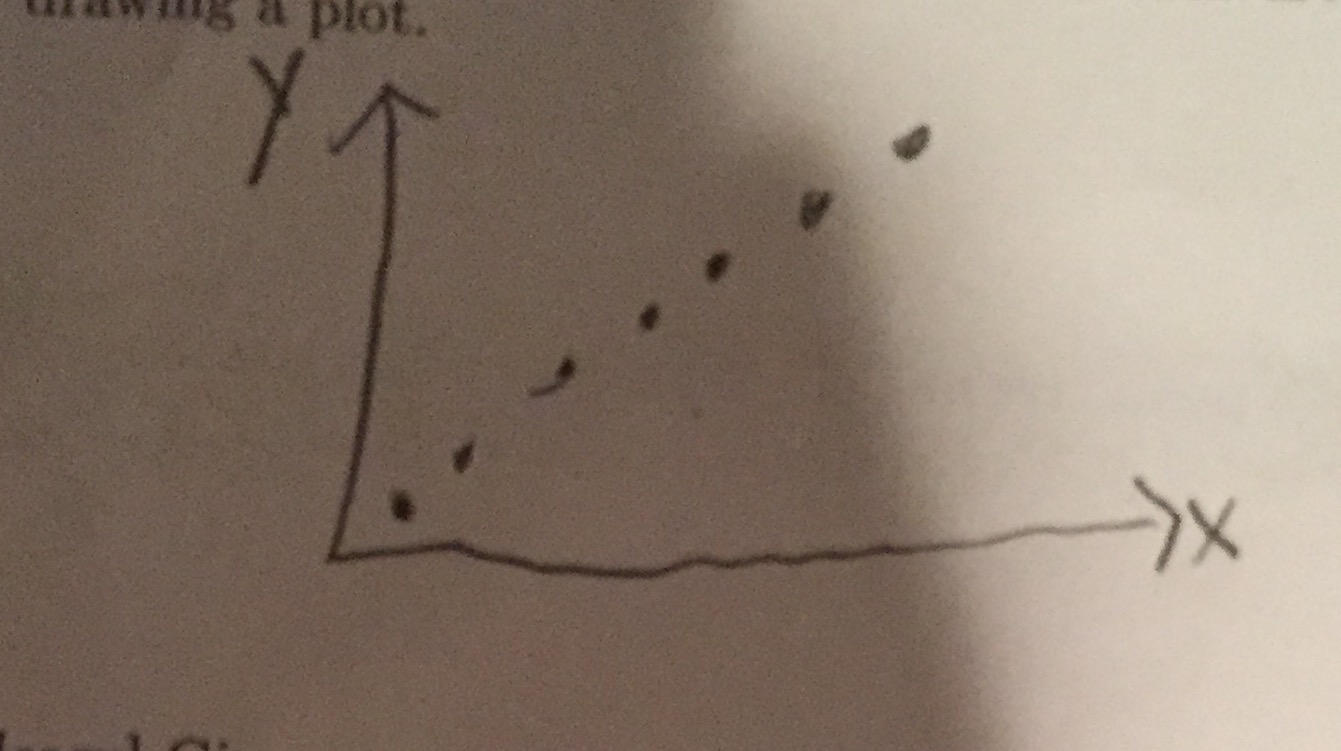
\includegraphics[width=3.8in]{prob3a.jpg}
\end{figure}



\easysubproblem{Give an example of two variables that are not correlated but are associated by drawing a plot.}\spc{10}
\begin{figure}[htp]

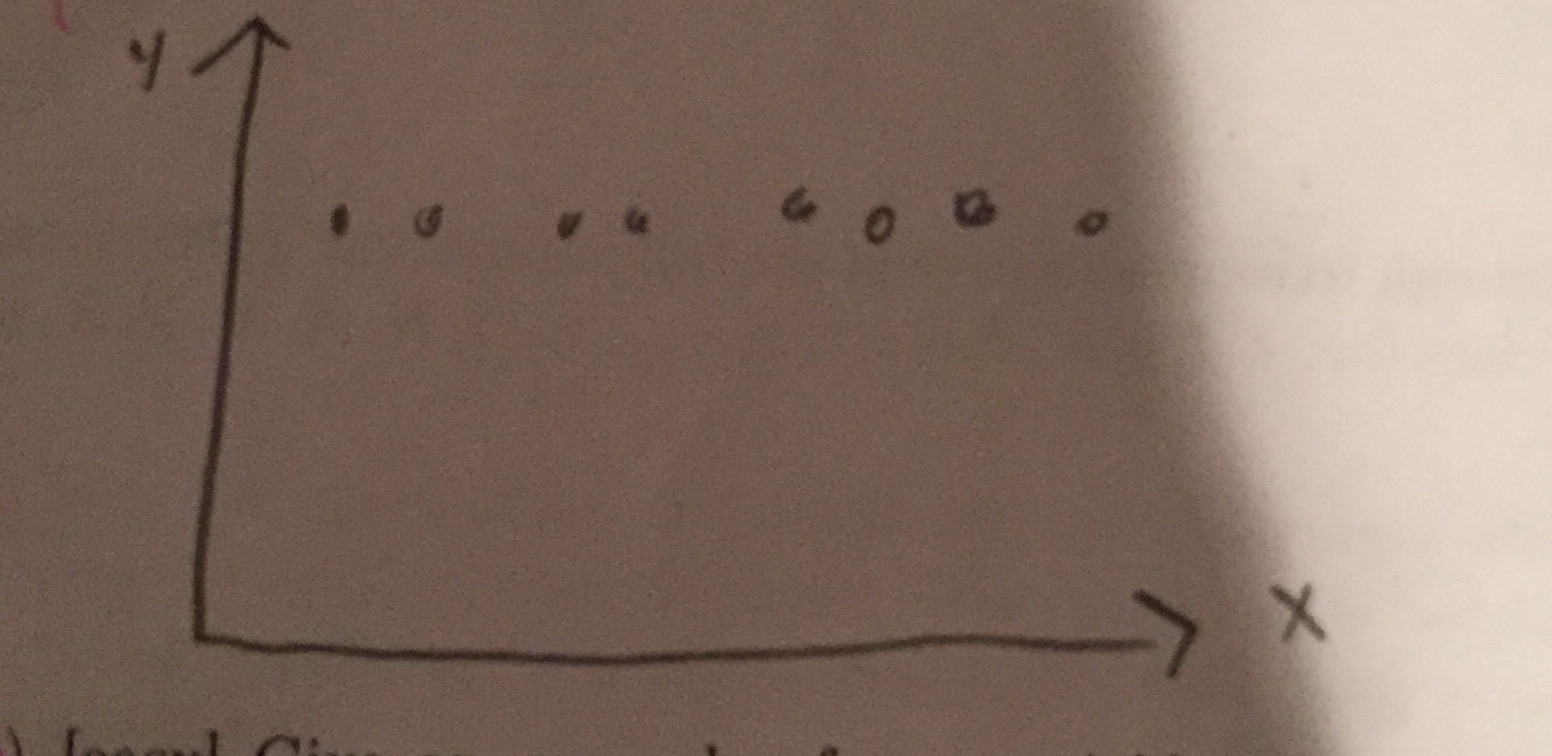
\includegraphics[width=3.8in]{prob3b.jpg}
\end{figure}

\easysubproblem{Give an example of two variables that are not correlated nor associated by drawing a plot.}\spc{4}
\begin{figure}[htp]

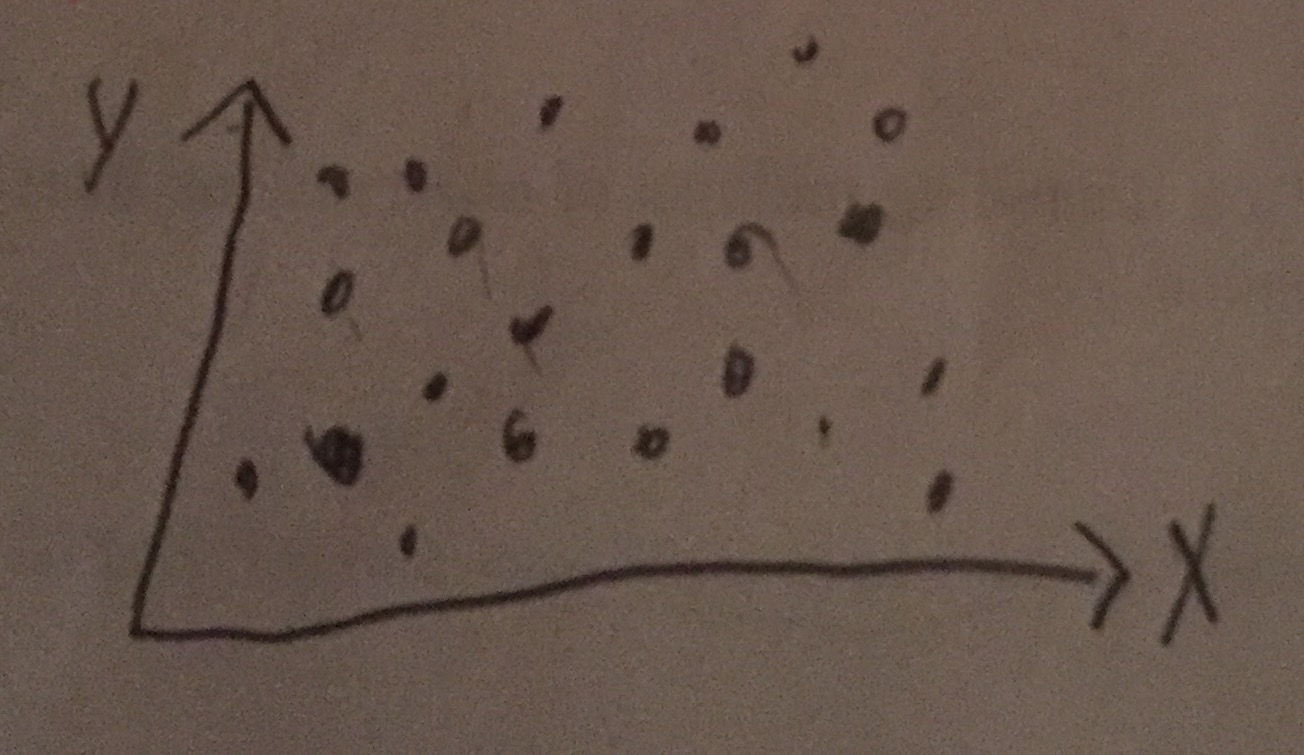
\includegraphics[width=3.8in]{prob3c.jpg}
\end{figure}

\easysubproblem{Can two variables be correlated but not associated? Explain.}\spc{4}
No. Correlation is a type of association.
\end{enumerate}
\newpage
\problem{These are questions about multivariate linear model fitting using the least squares algorithm.}
\begin{enumerate}

\hardsubproblem{Derive $\partialop{\c}{\c^\top A \c}$ where $\c \in \reals^n$ and $A \in \reals^{n \times n}$ but \textit{not} symmetric. Get as far as you can.}\spc{8}
\begin{equation*}
A\vec{c}= \begin{bmatrix}
a_{11}c_1+a_{12}c_2\cdots+a_{1n}c_n\\
a_{21}c_1+a_{22}c_2\cdots+a_{2n}c_n\\
\vdots\\
a_{n1}c_1+a_{n2}c_2\cdots+a_{nn}c_n
\end{bmatrix}\in\mathbb{R}^{n\times1}
\end{equation*}
Then \begin{equation*}
\vec{c}^T(A\vec{c})=c_1(a_{11}c_1+a_{12}c_2\cdots+a_{1n}c_n)+c_2(a_{21}c_1+a_{22}c_2\cdots+a_{2n}c_n)\cdots+c_n(a_{n1}c_1+a_{n2}c_2\cdots+a_{nn}c_n)
\end{equation*}
Take derivative with respect to $c_1$\begin{eqnarray*}
\frac{\partial}{\partial c_1}=(2a_{11}c_1+a_{21}c_2\cdots+a_{1n}c_n)+a_{21}c_2+a_{31}c_3\cdots+a_{n1}c_n\\=2a_{11}c_1+c_2(a_{12}a_{21})+c_3(a_{13}a_{31})\cdots+c_n(a_{1n}a_{n1})
\end{eqnarray*}
Take derivative with respect to $c_2$\begin{eqnarray*}
\frac{\partial}{\partial c_2}=(2a_{22}c_2+a_{21}c_1\cdots+a_{2n}c_n)+a_{12}c_1+a_{32}c_3\cdots+a_{n2}c_n\end{eqnarray*}

\easysubproblem{Given matrix $X \in \reals^{n \times (p+1)}$, full rank and first column consisting of the $\onevec_n$ vector, rederive the least squares solution $\b$ (the vector of coefficients in the linear model shipped in the prediction function $g$). No need to rederive the facts about vector derivatives.}\spc{10}%check answer

\begin{equation*}
SSE=\sum\limits_{i=1}^n(\vec{y_i}-\vec{\hat{y_i}})^2
 \end{equation*}
 which we can rewrite as \begin{equation*}
 (\vec{y}-\vec{\hat{y}})^T(\vec{y}-\vec{\hat{y}})=(\vec{y}^T-\vec{\hat{y}}^T)(\vec{y}-\vec{\hat{y}})
 \end{equation*}
 Foil
 \begin{equation*}
 \vec{y}^T\vec{y}-\vec{y}^T\vec{\hat{y}}-\vec{\hat{y}}^T\vec{y}+\vec{\hat{y}}^T\vec{\hat{y}}
\end{equation*}
Replace $\vec{y}^T\vec{\hat{y}}=\vec{y}\vec{\hat{y}}^T$
\begin{equation*}
\vec{y}^T\vec{y}-2\vec{y}\vec{\hat{y}}^T+\vec{\hat{y}}^T\vec{\hat{y}}
\end{equation*}
Replace $\vec{\hat{y}}=X\vec{w}$
\begin{equation*}
SSE=\vec{y}^T\vec{y}-2\vec{y}(X\vec{w})^T+(X\vec{w})^T(X\vec{w})
\end{equation*}
Take partials
\begin{equation*}
\frac{\partial}{\partial\vec{w}}[SSE]=\frac{\partial}{\partial\vec{w}}[\vec{y}^T\vec{y}]-2\frac{\partial}{\partial\vec{w}}[\vec{y}X^T\vec{w}^T]+\frac{\partial}{\partial\vec{w}}[X^TX\vec{w}^T\vec{w}]
\end{equation*}
\begin{equation*}
\frac{\partial}{\partial\vec{w}}[SSE]= \vec{0}_{p+1}-2X^T\vec{y}+2X^TX\vec{w}
\end{equation*}
Set $\frac{\partial}{\partial\vec{w}}[SSE]=0$, factor out the 2
\begin{align*}
-X^T\vec{y}+X^TX\vec{w}=0 \\
X^TX\vec{w}=X^T\vec{y}
\end{align*}
Since $X$ has full rank $p+1$, we know that $X^TX$ is invertible, and Let $\vec{w}=\vec{b}$
\begin{equation*}
\vec{b}=(X^TX)^{-1}X^T\vec{y}
\end{equation*}


\intermediatesubproblem{Consider the case where $p = 1$. Show that the solution for $\b$ you just derived is the same solution that we proved for simple regression in Lecture 8. That is, the first element of $\b$ is the same as $b_0 = \ybar - r \frac{s_y}{s_x}\xbar$ and the second element of $\b$ is $b_1 = r \frac{s_y}{s_x}$.} \spc{10}

\begin{eqnarray}
b_1=r\frac{s_y}{s_x}=\frac{(n-1)S_{xy}}{(n-1)S_{xx}}=\frac{\sum\limits_{i=1}^nx_iy_i-n\bar{x}\bar{y}}{\sum\limits_{i=1}^nx_i^2-n\bar{x}^2}\\
b_0=\bar{y}-r\frac{s_y}{s_x}\bar{x}
\end{eqnarray}
 From the previous question, we know that $\vec{b}=(X^TX)^{-1}X^T\vec{y}$ and since $p=1$, $X\in\mathbb{R}^{n\times2}$ 
\begin{equation*}
X=\begin{bmatrix}1 && x_1\\1 && x_2\\\cdots\\1 && x_n\end{bmatrix}\\ 
X^T= \begin{bmatrix}1 && 1 && \cdots && 1\\x_1 && x_2 && \cdots && x_n\end{bmatrix} \\
\vec{y}=\begin{bmatrix}y_1\\y_2\\\vdots\\y_n\end{bmatrix}
\end{equation*}
using  (note:$\sum\limits_{i=1}^ny_i=n\bar{y}$) 
\begin{equation*}X^T\vec{y}=
\begin{bmatrix}1&&1&&\cdots&&1\\x_1&&x_2&&\cdots&&x_n\end{bmatrix}
\begin{bmatrix}y_1\\y_2\\\vdots\\y_n\end{bmatrix}=
\begin{bmatrix}\sum\limits_{i=1}^ny_i\\\sum\limits_{i=1}^nx_iy_i \end{bmatrix}=
\begin{bmatrix}n\bar{y}\\\sum\limits_{i=1}^nx_iy_i \end{bmatrix}
\end{equation*}

Now mutiply(note:$\sum\limits_{i=1}^nx_i=n\bar{x}$) \begin{equation*}X^TX= \begin{bmatrix}1 && 1 && \cdots && 1\\x_1 && x_2 && \cdots && x_n\end{bmatrix}
\begin{bmatrix}1 && x_1\\1 && x_2\\\cdots\\1 && x_n\end{bmatrix} = 
\begin{bmatrix}n && \sum\limits_{i=1}^nx_i\\\sum\limits_{i=1}^nx_i && \sum\limits_{i=1}^nx_i^2\end{bmatrix}=
\begin{bmatrix}n &&n\bar{x}\\n\bar{x}&&\sum\limits_{i=1}^nx_i^2\end{bmatrix}\end{equation*}
Since X has full rank we can take the inverse of it(note: $S_{xx}=\sum\limits_{i=1}^nx_i^2-n\bar{x}^2$)\begin{equation*}
\det{X^TX}=n\sum\limits_{i=1}^nx_i^2-(n\bar{x})^2=n(\sum\limits_{i=1}^nx_i^2-n\bar{x}^2)=nS_{xx}\end{equation*}
The inverse is then \begin{equation*}
(X^TX)^{-1}=\frac{1}{nS_{xx}}\begin{bmatrix}
\sum\limits_{i=1}^nx_i^2&&-n\bar{x}\\
-n\bar{x}&&n
\end{bmatrix}=\frac{1}{S_{xx}}\begin{bmatrix}
\frac{1}{n}\sum\limits_{i=1}^nx_i^2&&-\bar{x}\\
-\bar{x}&&1\end{bmatrix}\end{equation*}
Now we have  \begin{equation*}
\vec{b}=(X^TX)^{-1}X^T\vec{y}=\frac{1}{S_{xx}}\begin{bmatrix}
\frac{1}{n}\sum\limits_{i=1}^nx_i^2&&-\bar{x}\\
-\bar{x}&&1
\end{bmatrix}\begin{bmatrix}n\bar{y}\\\sum\limits_{i=1}^nx_iy_i \end{bmatrix}=
\frac{1}{S_{xx}}\begin{bmatrix}
\frac{1}{n}(\sum\limits_{i=1}^nx_i^2)(n\bar{y})-\bar{x}\sum\limits_{i=1}^nx_iy_i\\
-\bar{x}n\bar{y}+\sum\limits_{i=1}^nx_iy_i
\end{bmatrix}
\end{equation*}
\begin{equation*}
\vec{b}=\frac{1}{\sum\limits_{i=1}^nx_i^2-n\bar{x}^2}\begin{bmatrix}
\bar{y}\sum\limits_{i=1}^nx_i^2-\bar{x}\sum\limits_{i=1}^nx_iy_i\\
\sum\limits_{i=1}^nx_iy_i-n\bar{x}\bar{y}
\end{bmatrix}
\end{equation*}
\begin{equation}
b_1=\frac{\sum\limits_{i=1}^nx_iy_i-n\bar{x}\bar{y}}{\sum\limits_{i=1}^nx_i^2-n\bar{x}^2}=r\frac{s_y}{s_x}
\end{equation}
EquatioN 3 matches equation 1 from above\\
Now sub $b_1$ into the equation for $b_0$
\begin{equation}
b_0=\frac{\bar{y}\sum\limits_{i=1}^nx_i^2-\bar{x}\sum\limits_{i=1}^nx_iy_i}{\sum\limits_{i=1}^nx_i^2-n\bar{x}^2}=\bar{y}-\bar{x}r\frac{s_y}{s_x}
\end{equation}


\easysubproblem{If $X$ is rank deficient, how can you solve for $\b$? Explain in English.} \spc{2}

Since $X$ is rank deficient, $b$ is not in the column space of $X$. Instead of solving exactly for $b$, we could find the element in column space of $X$ that is "closest" to $b$, which is its' projection. So we are looking for the hat matrix that gives us $H\vec{y}=Proj_b(X)$

\hardsubproblem{Prove $\rank{X} =\rank{X^\top X}$.}\spc{6}

\hardsubproblem{Given matrix $X \in \reals^{n \times (p+1)}$, full rank and first column consisting of the $\onevec_n$ vector, now consider cost multiples (\qu{weights}) $c_1, c_2, \ldots, c_n$ for each mistake $e_i$. As an example, previously the mistake for the 17th observation was $e_{17} := y_{17} - \hat{y}_{17}$ but now it would be $e_{17} := c_{17} (y_{17} - \hat{y}_{17})$.  Derive the weighted least squares solution $\b$. No need to rederive the facts about vector derivatives. Hints: (1) show that SSE is a quadratic form with the matrix $C$ in the middle (2) Split this matrix up into two pieces i.e. $C = C^{\half} C^{\half}$, distribute and then foil (3) note that a scalar value equals its own transpose and (4) use the vector derivative formulas.}\spc{20}


\hardsubproblem{If $p=1$, prove $r^2 = R^2$ i.e. the linear correlation is the same as proportion of sample variance explained in a least squares linear model.}\spc{6}


\intermediatesubproblem{Prove that the point $<1,\xbar_1, \xbar_2, \ldots, \xbar_p, \bar{y}>$ is a point on the least squares linear solution.}\spc{13}

\end{enumerate}

\problem{These are questions related to the concept of orthogonal projection, QR decomposition and its relationship with least squares linear modeling.}

\begin{enumerate}

\easysubproblem{Consider least squares linear regression using a design matrix $X$ with rank $p + 1$. What are the degrees of freedom in the resulting model? What does this mean?}\spc{3}


\intermediatesubproblem{If you are orthogonally projecting the vector $\y$ onto the column space of $X$ which is of rank $p + 1$, derive the formula for $\proj{\colsp{X}}{\y}$. Is this the same as the least squares solution?}\spc{6}

Let $\colsp{X}=[X_1, X_2\cdots, X_{p+1}]\in\mathbb{R}^{n\times{p+1}}$\\
Notes \begin{itemize}
\item (1) $\y=\proj{\colsp{X}}{\y}+\ev\\ \Rightarrow\ev=\y-\proj{\colsp{X}}{\y}$
\item (2)$\ev\cdot\proj{\colsp{X}}{\y}=\vec{0}$ and $\ev\cdot\colsp{X}=\vec{0}$
\end{itemize}
Since $\y$ is being orthogonally projected onto the column space of $X$, we know that $\proj{\colsp{X}}{\y}\in\colsp{X}$. In other words, $\exists$ a scalar $\wv$ s.t \begin{equation}
\proj{\colsp{X}}{\y}=w_1X_1+w_2X_2\cdots w_{p+1}X_{p+1}=X\wv
\end{equation}
By note 1 $\ev=\y-X\wv$ and by note 2 $X^T(\y-X\wv)=\vec{0}$
\begin{eqnarray*}
X^T(\y-X\wv)=\vec{0}\\
X^T\y-X^TX\wv=\vec{0}\\
X^T\y=X^TX\wv
\end{eqnarray*}
Since $X$ has full rank $p+1$, $X^TX$ is also of full rank which means we can take the inverse firecetly\begin{equation}
(X^TX)^{-1}X^T\y=\wv
\end{equation}
Now plug $\wv$ into equation 1 and we get \begin{equation}
\proj{\colsp{X}}{\y}= X(X^TX)^{-1}X^T\y
\end{equation}
Which is the same as the least squares solution.


\hardsubproblem{We saw that the perceptron is an \textit{iterative algorithm}. This means that it goes through multiple iterations in order to converge to a closer and closer $\w$. Why not do the same with linear least squares regression? Consider the following. Regress $\y$ using $\X$ to get $\yhat$. This generates residuals $\e$ (the leftover piece of $\y$ that wasn't explained by the regression's fit, $\yhat$). Now try again! Regress $\e$ using $\X$ and then get new residuals $\e_{new}$. Would $\e_{new}$ be closer to $\zerovec_n$ than the first $\e$? That is, wouldn't this yield a better model on iteration \#2? Yes/no and explain.}\spc{10}

Each residual, $e_i$, is calculated by $e_i=y_i-\hat{y}_i$ where $\hat{y}_i=X_iw_i$. Hence $\vec{e}$ is dependent on X. Running a regression on dependent variables will return a smaller error rate than if you ran the regression on independent variables. So, yes, this process will yield a better model on iteration 2.

\intermediatesubproblem{Prove that $Q^\top = Q^{-1}$ where $Q$ is an orthonormal matrix such that $\colsp{Q} = \colsp{X}$ and $Q$ and $X$ are both matrices $\in \reals^{n \times (p+1)}$. Hint: this is purely a linear algebra exercise.}\spc{10}

Calculate $Q^TQ=\begin{bmatrix}
\leftarrow q_1 \rightarrow\\
\leftarrow q_2 \rightarrow\\
\vdots\\
\leftarrow q_{p+1} \rightarrow\\
\end{bmatrix}\begin{bmatrix}
\uparrow & \uparrow & \cdots & \uparrow\\
q_1 & q_2 & \cdots & q_{p+1}\\
\downarrow & \downarrow & \cdots & \downarrow
\end{bmatrix}=\begin{bmatrix}
1 & 0 & \cdots & 0\\
0 & 1 & \cdots & 0\\
\ddots\\
0 & 0 & \cdots & 1
\end{bmatrix}$
So $Q^TQ=I_{p+1}$. Linear algebra rules tell us that if we have a vector times its' own transpose that equals the identity matrix, the transpose of that matrix must be equal to the inverse. In basic math, if we have $xy=1$, without loss of generality, $x=y^{-1}$. Here we just have the vector version of this relationship. Hence $Q^T=Q^{-1}$ 

\intermediatesubproblem{Prove that the least squares projection $H = \XXtXinvXt$ is the same as $QQ^\top$.}\spc{10}

\intermediatesubproblem{Prove that an orthogonal projection onto the $\colsp{Q}$ is the same as the sum of the projections onto each column of $Q$.}\spc{10}


\hardsubproblem{Trouble in paradise. Prove that the SSE of a multivariate linear least squares model always decreases (equivalently, $R^2$ always increases) upon the addition of a new independent predictor. Keep in mind this holds true even if this new predictor has no information about the true causal inputs to the phenomenon $y$.}\spc{12}

\intermediatesubproblem{Why is this a bad thing? Explain in English.}\spc{3}



\extracreditsubproblem{Prove that $\rank{H} =\tr{H}$.}\spc{-0.5}

\end{enumerate}


\end{document}
